\documentclass[12pt, a4paper]{article}

\usepackage[T1]{fontenc}
\usepackage[utf8]{inputenc}
\usepackage{libertinust1math}

\usepackage{csquotes}
\usepackage[english]{babel}
\usepackage[backend=biber, style=apa, sorting=nyt]{biblatex}
\addbibresource{thesis.bib}

\usepackage{graphicx}
\usepackage{subcaption}
\graphicspath{{./assets/}}

\title{Thesis draft}
\author{Joshua Megnauth}
\date{\today}

\begin{document}
\maketitle

\section{Introduction: Reddit, gamers, and social networks}
Gaming is an omnipresent artistic medium enjoyed by a plurality of Americans. Research from the \textit{Entertainment Software Association} (E.S.A.) has found that about 65\% of American adults play video games. About 46\% of said gamers are female (\cite{esagamers}). The E.S.A.'s research counters the tired trope of gamers as young, immature boys. Despite the prevalence and diversity of gamers academia is woefully behind on ludology, the study of gaming. Gaming lacks the prestige of other artistic entertainment media such as books, music, and film. An interested party may find texts on the innovations of Allen Ginsberg's poem \textit{Howl} or Sonic Youth's \textit{Daydream Nation} while scarcely finding an academic article on the contributions of the video game \textit{Doom}. 

Ludology is as exciting as fields such as A.I. despite lacking the selfsame effervescence. In other words, ludology may be studied from many different angles. Political sociologists would find much to mine from the philosophical schisms in the gaming community. Recent grassroots movements to push for more representation in video games spawned a revanchist and sexist counter movement. Besides the political, sociologists may write ethnographies of the online communities or interactions that occur within gaming. Mark Chen's \textit{Leet Noob: The Life and Death of an Expert Player Group in 'World of Warcraft'} is a study of a group of gamers who tackle dungeons in \textit{World of Warcraft}. Chen writes from the perspective of both a gamer and a social scientist to apply theories such as social and cultural capital, actor-network theory, social construction, et cetera to the video game (\cite{chenwow}). The list above is clearly not exhaustive. However, I'd like to mention, as an aside, that online communities are transient; ignoring ludology risks permanently missing out on an aspect of culture.

My thesis focusses on the intersection between network science via the social network Reddit and video games. I am particularly interested in the distribution of gamers across subreddits. Reddit and the related terminology will be explained below. I hypothesize that gamers are more likely to post on multiple gaming subreddits (that is, gamers are more likely to have a community that spans across subreddits). Analyzing the network dispersion of gamers is useful for both the social sciences as well as marketing. Network science is concerned with the spread of information by virtue of its focus on ties. Users who post on multiple subs may pass information across subreddits.

My guiding principle is thus to use my statistical and computing skill coupled with my domain knowledge of video games in order to contribute to ludology. Previous studies on gaming lack domain expertise while exhibiting logical fallacies---both of which seem to be caused by the hermetic world of academia. More proper ludology needs to seed the field until the study of video games resembles writing on music or films. 

An anecdote engendered my thesis. I've observed; anecdotally, like many others; that nerds of a feather tend to flock together. Gamers tend to share a sample from a common set of interests such as anime, wrestling, technology, certain tastes in music, et cetera. This observation is far from holistic---meaning, gamers do not adopt all of the same traits, and clearly not every person who watches wrestling, for example, is a gamer. However, the basic observation led to my thesis. My research is not seeking to answer that question specifically, but my thesis may provide the groundwork toward studying that larger topic. Gamers may preferentially attach to other gamers or to other ostensibly related subjects such as anime or eSports. Either conclusion---that gamers preferentially attach or not---is useful for ludology. 

\section{Background: Social network analysis}

\subsection{A digital approach}
My goal is to contribute to both ludology as well as studies of Reddit. Gaming by virtue is a heavily technological affair. Gamers are often only lightly insulated from technology. For example, anyone who follows gaming news would likely run into computer terms. Even gamers who do not follow gaming news would run into patches, lag, bugs, or have to know how to connect their consoles to the internet, et cetera. Gaming is unlike television or cable in that video games have a strongly "digital native" feel---especially for P.C. (computer) gamers. Gamers discuss video games online on platforms such as Reddit or news sites with forums and comment systems. The culmination of these "techy" qualities does not imply that all gamers are computer scientists but that they are generally reasonably comfortable with technology. All of this is to say that a network analysis focussing on gamers and Reddit is sensible because of the focus on internet media.

\subsection{Why video games?}
Gamers and ludology, as discussed earlier, are legitimate areas of study that are largely ignored by academia as well as having an image problem regardless of gaming's prevalence. Gaming as a medium is sometimes strangely maligned as coercing individuals toward violence. In 2019, President Donald Trump as well as Kevin McCarthy and Dan Patrick, both Republican politicians, scapegoated video games as reported by an article in the New York \textit{Times}. The article explains that games are often blamed for shootings despite the lack of causal evidence. The American Psychological Association, according to the \textit{Times}, is that video games and violence are not linked. Dr. Chris Ferguson of the A.P.A. humorously mentioned that the data linking bananas to suicide are about the same as those data connecting video games and other media to violence (\cite{drapernyt0819}).

Most research published on gaming is cursory while also lacking domain knowledge on the subject. A search through databases that compile articles, such as JSTOR, on video games shows that research is decidedly lacking in imagination as they mostly focus on the antiquated violence question. One such article published in \textit{Frontiers of Psychology} exhibits a very flawed methodology in studying gamers. The researchers use an imbalanced and relatively small random sample that skews young and male. Females consisted of a scant 15\% of their sample. The writers justified the skewed sample by referencing a two decade old paper despite publishing their article in 2019 and using recent sources otherwise (\cite{badresearch}). Research from the NPD Group corroborates what the E.S.A. found and gamers already know: about half of gamers are women and more females own the 3DS, Wii U, and Nintendo Switch than males (\cite{npdgamers}). Beyond the poor sampling the research heavily relies on p-values without associated effect sizes. Furthermore, the basis for the study is intrinsically flawed. Gamers are a wide social unit. We would not sample around 3000 music buffs in order to see if "problematic music listening" is associated with "poor psychological functioning."

\subsection{What is Reddit?}
\begin{figure}[h!]
  \centering
  \begin{subfigure}[b]{0.4\linewidth}
    
\includegraphics[width=\linewidth]{reddit_rust_comments.png}
    \caption{Comments on an /r/rust thread}
  \end{subfigure}
  \begin{subfigure}[b]{0.4\linewidth}
    
\includegraphics[width=\linewidth]{reddit_ps4.png}
    \caption{/r/ps4 threads (old scheme)}
  \end{subfigure}
  \begin{subfigure}[b]{0.4\linewidth}
    
\includegraphics[width=\linewidth]{reddit_pcgaming.png}
    \caption{/r/pcgaming threads (new scheme)}
  \end{subfigure}
  \label{fig:redditexamples}
  \caption{Examples of Reddit, a forum-like social network}
\end{figure}
Reddit is a social network reminiscent of the forums and bulletin board systems (B.B.S.) of the past. Reddit is designed for lengthy deliberation, or at least facilitates it, which is like forums and unlike Twitter or Facebook. Subreddits is Reddit parlance for a community which is similar to a forum. Pseudonymous users may post or reply to discussion topics. Individual subreddits are moderated by screened volunteers from the community; rules are enforced and users may not be able to post if their reputation---known as karma---is too low. Needless to say, Reddit's structure engenders higher quality content---generally speaking at least as Reddit is also home to lengthier discussions on puerile matters. Reddit users, who are pseudonymous, are known by the demonym Redditors.

Reddit reflects gaming's preeminence via \textit{many} the many subreddits on the topic; individual consoles, series, genres, abstruse memes, as well as technological concepts such as emulation all have incredibly active subs. Reddit is the seventeenth most popular site in the world according to \textit{Alexa}, a subsidiary of Amazon that collects internet data. The social network's position varies from day to day but remains consistently high. Reddit is ahead of several prominent sites such as Netflix, Hulu, Crunchyroll, Instagram, Microsoft's site, Live (Outlook), Twitch, Bing, eBay, AliExpress, and others. Reddit is mainly behind sites such as Chinese social networks such as Weibo as well as Google and YouTube \cite{alexatop}. The largest gaming subreddit on Reddit, \textit{/r/gaming}, is the fourth most popular total which places \textit{gaming} above the subreddits for music, sports, relationships, movies, news, gifs, cats, cute pictures, books, programming, et cetera. In fact, the only subreddit more popular than \textit{gaming} that is \textit{not} a default subscription is \textit{/r/funny}. The subreddit for \textit{League of Legends}, a single video game, is the sixtieth most popular subreddit \cite{redditlist}.

Redditors may post on as many or as little subreddits as they wish. For example, a user may post on the subreddits for PlayStation 4, P.C. gaming, Linux, and the systems programming language, Rust. Another user may frequent the subs for K-Pop, anime, and the Nintendo Switch.

\subsection{Big data---Volume, Variety, and Velocity}
Graph theory does not imply big data, but network science scales well to a high number of observations.Computational social science naturally trends towards big data, such as large graphs or natural language processing. Amir Gandomi and Haider Murtaza argue that the term "big data" is often misunderstood which may impact comprehending a big data project. Big data is traditionally defined by the three Vs: volume, variety, and velocity. Volume is the most straightforward of the three concepts. The "big" in big data suggests a generous amount of information. Volume is simply that---\text{a lot} of data \cite{gandomiamir2015}.

Variety and velocity are the more interesting of the three Vs. Big data is often raw and heterogeneous. Unlike the nicely structured flat files data are often distributed as, the majority of existing data are unstructured and multiformat \cite{gandomiamir2015}. For example, Twitter data would likely arrive in a set of different languages with varying levels of grammar, zeitgeist and context specific references, embedded multimedia, retweets, et cetera. With that said, Twitter data may still be pulled from a clean API which means that Tweets are hardly the most unstructured data a scientist would find. Variety, thus, also refers to the format of data; different image or video formats must be handled, and unstructured data must be appropriately stored as well. 

Big data is not only intractably diverse but they are also produced at a high velocity \cite{gandomiamir2015}. For example, consider all of the data gathered by voice processing systems such as Siri, Alexa, or Google Assistant. Simply browsing the internet, even with JavaScript and DNS blocking, produces an enormous amount of data. Cellphones collect data more or less constantly, especially with more programs/apps in use. \footnote{Data are collected in a manner so megalomaniacal that the European Union instituted the \text{General Data Protection Regulation} to protect the privacy of E.U. citizens.}

The three Vs galvanized the use of certain techniques of gathering and analyzing data. Natural Language Processing, graph theory, unstructured databases, clustering, et cetera are not new, but big data have made such techniques both more viable as well as more necessary. NLP, neural networks, as well as computer vision are hotshot fields of data science more generally as well as the computational social sciences due to the prevalence of so much data. After all, what else would we do with said data \cite{gandomiamir2015}? 

Finally, social network analysis is at least a century old but big data presents new applications. 

\subsection{Weak ties in social networks}
To do\cite{granovetter1973}

\subsection{Co-posting networks via Reddit}
To do \cite{}

\section{Methodology}

\begin{figure}[h!]
  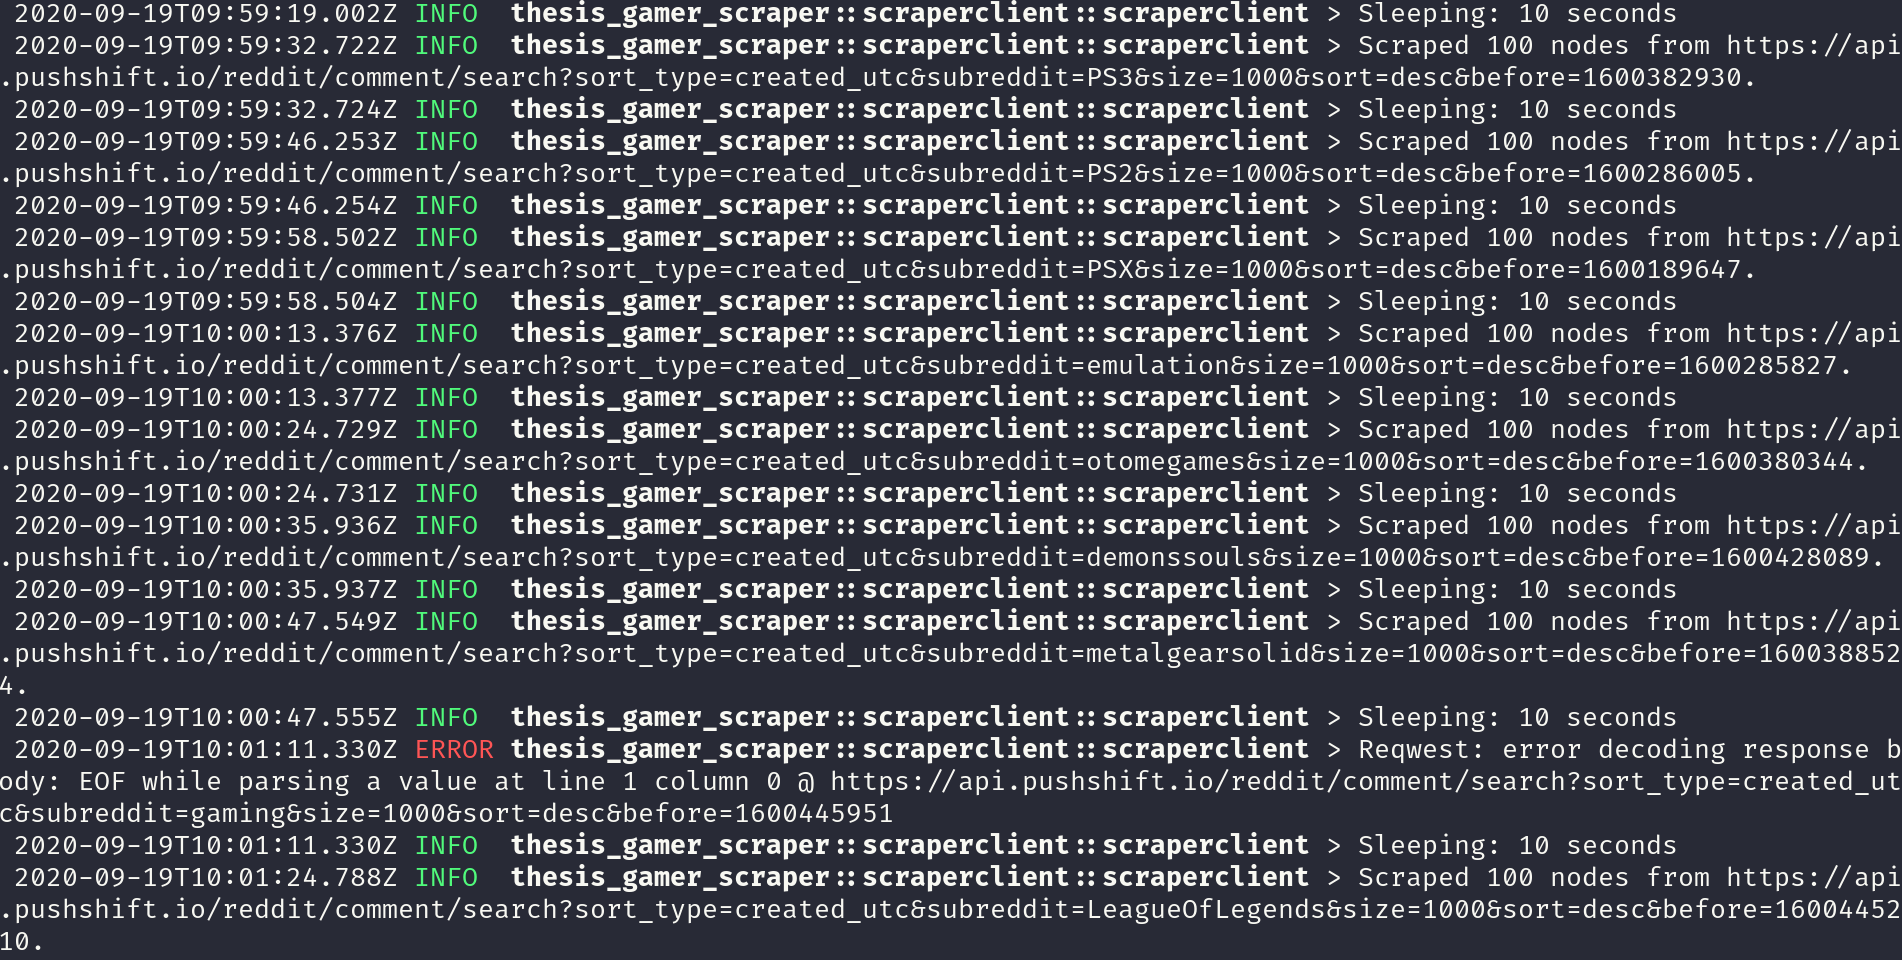
\includegraphics[width=\linewidth]{scraper_at_work.png}
  \caption{Scraper hard at work}
  \label{fig:workingscraper}
\end{figure}

My research project requires relatively recent data as well as observations relevant to video games. Researchers in the computational social sciences seem to trend toward gathering their own data. The internet is a dynamic space of constant data production. Structured data may be limited or flawed for many topics, including ludology. Scraping data allows computational social scientists to gather raw, unpasteurized data rather than relying on old, static sources. A survey, for example, is saliently flawed for gamers because conducting one properly would likely require a large sample across a wide span of ages as well as capture gamers who play on different platforms. Scraping data seems both more reliable as well as more direct in a case like that as well as for my project.

While large Reddit data sets exist via the \textit{Stanford Network Analysis Project} as well as \textit{Kaggle}, scraping data from Reddit is not too difficult due to the open Reddit API \cite{redditapi}. Bindings for Python exist via \textit{PRAW} as well. However, the Reddit API imposes several restrictions and requires an account to use properly as well. The restrictions are reasonable due to Reddit's high traffic: rapacious scrapers may hammer the site and associated Content Delivery Networks. Caching services, such as the open source Pushshift, aims to alleviate the stress caused by scrapers as well as provide a more convenient API \cite{pushshiftapi}. I opted for Pushshift to gather my data due to its flexibility.

My scraper gathers \textit{N} Node-Edge pairs from a provided list of subreddits. I wrote the scraper in the systems programming language, Rust, and the source code is available on GitHub\footnote{https://github.com/joshuamegnauth54/thesis\_gamer\_scraper}. My program's high level logic is as follows: 

\begin{enumerate}
  \item Collect 100 nodes with associated metadata from a subreddit. Each observation contains the Redditor name, epoch timestamps, and subreddit name.
  \item Paginate by setting the \textit{before} API parameter to the earliest timestamp from the recent scrape of 100 nodes.
  \item Add each gathered node to a hash set which precludes duplicate observations.
  \item Repeat steps one through three for the set of subreddits in a round robin manner.
  \item Repeat steps one through four until \textit{N} is reached.
  \item Remove deleted users and automoderator replies.
  \item Hash all of the Redditor names with SHA256 at an attempt at privacy\footnote{Very little of the data sets found online actually hashed the user names as the information is all public. However, hashing at least adds a minimum layer of privacy.}.
  \item Save everything to a CSV.
\end{enumerate}

My data set\footnote{Available here: https://github.com/joshuamegnauth54/GamerDistributionThesis2020/data} contains about 78,000 observations gathered via the logic above.

\printbibliography

\end{document}
